\clearpage
\section{在编辑器里运行 Vulkan}\label{impl:entry}
用 Vulkan 打开 RedflagForge，首先看到 Sponza 中庭。右侧 Lighting 面板默认选中 Lit，石柱与挂毯受场景里的三盏点光源照明。左侧选择一盏灯，可以在 Inspector 里调整颜色、强度和位置。中间的 Scene 视图使用编辑相机，Game 视图使用场景中勾选「主相机」的相机。

\codewhere{运行命令}{tests/fetch_sponza.py}{模型下载与 Vulkan 启动}
\begin{lstlisting}
(*@\rhicomment{\# 首次运行时补齐中庭模型和贴图。}@*)
python tests/fetch_sponza.py
Set-Location RedflagForge
..\bin\Debug-windows-x86_64\RedflagForge\RedflagForge.exe --vulkan
\end{lstlisting}

下载脚本会补齐中庭模型和贴图。进入编辑器目录后再启动程序，场景、字体和贴图都从这个目录读取。省略 \code{--vulkan} 就使用 OpenGL。在新环境中，先安装 Visual Studio 的 C++ 工具与 Vulkan SDK，设置 \code{VULKAN\_SDK}，从仓库根目录运行 \path{GenerateProjects.bat}，打开解决方案构建 \code{RedflagForge}。本机使用 SDK 1.3.275.0。

\subsection{开窗前选择图形后端}
程序先在 \code{EntryPoint.h} 读取启动选项，再由 \code{WindowsWindow} 创建窗口。OpenGL 使用自己的上下文。选用 Vulkan 时，窗口将由另一套呈现机制显示画面，因此创建窗口前就要告诉 GLFW 使用 \code{GLFW\_NO\_API}。\code{VulkanContext} 随后找到能绘制并显示到该窗口的设备，准备可轮流显示的图像。

应用只在 \code{BeginFrame()} 成功取到图像后才让各层绘制。若用户把窗口最小化，本轮继续处理窗口消息。等窗口恢复，后端再按实际像素尺寸准备图像。这个判断留在窗口和上下文里，模型加载器就无需知道桌面窗口有多大。

\readings{源码位于 \path{Redflag/src/Platform} 下的 \path{Windows} 与 \path{Vulkan} 目录。\quad
\refitem{https://docs.vulkan.org/guide/latest/swapchain_semaphore_reuse.html}{Khronos · 窗口取图}}

\clearpage
\section{编辑器与照明设置}
\begin{center}
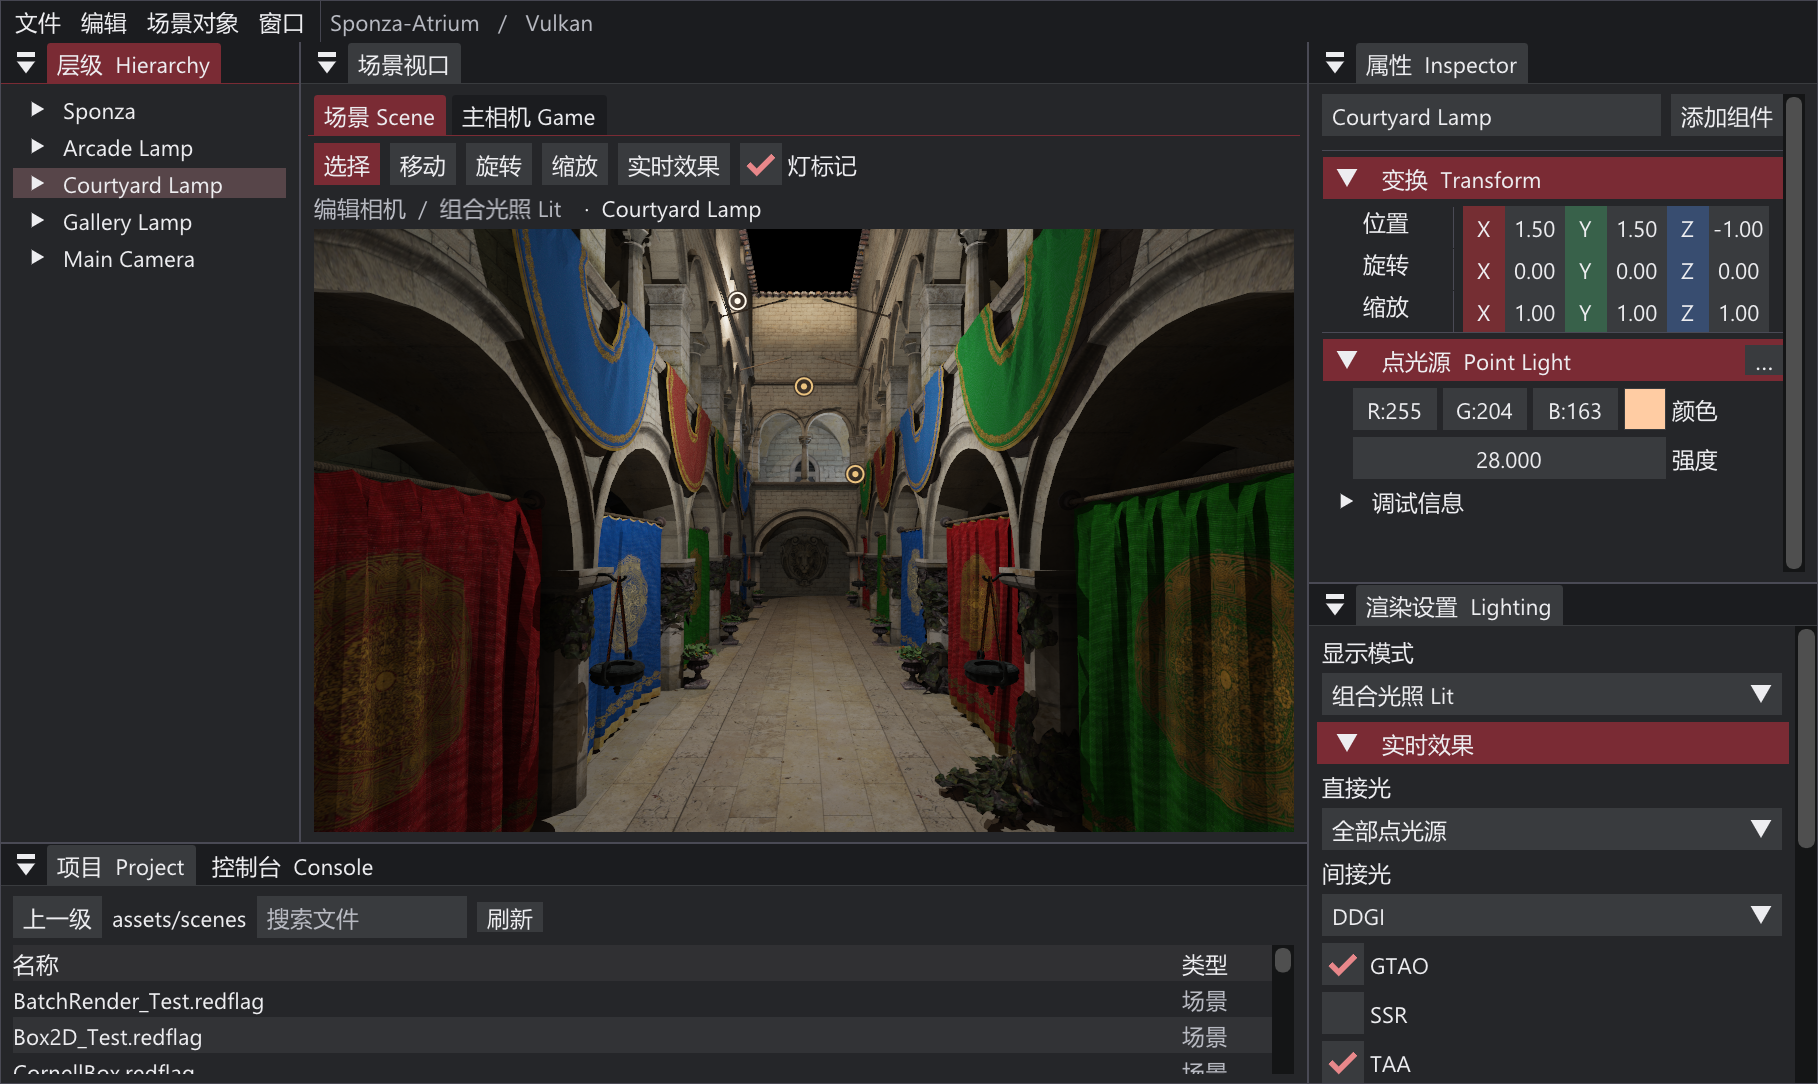
\includegraphics[width=\linewidth]{../../../output/rhi/editor-light-inspector.png}
\captionof*{figure}{在层级中选中中庭的 Courtyard Lamp 后，右侧显示这盏灯的位置、颜色与强度。场景视图中相应的灯标记呈金色。下方的「渲染设置」影响整个场景。}
\end{center}

调整灯光强度时，属性面板直接修改选中实体的 \code{PointLightComponent}。绘制下一帧时，\code{LightingPreview::Render} 从场景读取每盏灯的位置，并用颜色乘强度得到三通道的光照强度。发现灯光发生变化后，它丢弃先前积累的颜色，用新强度重新计算。两块面板因而各有一份明确的工作。属性面板负责改场景，渲染设置决定用哪种方法显示这批灯照出的画面。

「实时效果」可以从视口上方直接打开。它和右侧面板共用同一组设置，选择 DDGI、勾选 GTAO 后，\code{RenderLit} 便按下一页的顺序计算两者。「只显示直接光」可暂时查看直接照明。关掉即可恢复刚才的设置。保存时，模型、灯光和相机写入 \code{.redflag}，光照方法、采样数和效果参数写入同名的 \code{.render.yaml}。两份文件应一起移动。「只显示直接光」仅供当次比较，不写入场景。

\href{run:Redflag-Editor-Guide.pdf}{编辑器用户手册}附有选灯与切换光照的实拍步骤。

\readings{布局参考 Unity 官方手册中 Scene、Hierarchy、Inspector、Project 的使用习惯。\quad
\refitem{https://docs.unity3d.com/6000.0/Documentation/Manual/UsingTheSceneView.html}{Unity · 场景视图}\quad
\refitem{https://docs.unity3d.com/6000.0/Documentation/Manual/ProjectView.html}{Unity · 项目浏览器}}

\clearpage
\section{光照合成与场景面板的清晰度}
「组合光照 Lit」先算点光源直接照到表面的亮度，再加上已经照过别处、反射过来的一份光。以柱底为例，打开 GTAO 会压暗附近物体遮住的那部分间接光。灯光直射到柱面的一部分仍保留原来的亮度。勾选 SSR 后，屏幕空间反射会从已经合成的场景颜色中取样。开启体积雾时，雾先改变背景亮度。场景里有玻璃时，再用玻璃的朝向和折射率找背景像素。TAA 放在最后，将不同采样位置的颜色累积成当前显示的图。

\codewhere{流程伪代码}{RedflagForge/src/LightingPreview.cpp}{LightingPreview::RenderLit}
\begin{lstlisting}
direct   = RenderDirect(sceneLights);
indirect = RenderIndirect(scene, chosenMethod);
color    = direct + indirect * visibility;
(*@\rhicomment{// 反射和雾先改变背景，玻璃随后从那张图取色。}@*)
if (reflections) color = Reflect(color);
if (fog)         color = RenderFog(color);
if (glass)       color = CompositeTransparency(color);
if (taa)         color = Accumulate(color, history);
\end{lstlisting}

Native 让显卡为面板上的每个像素计算一个像素。把预览宽度改为 320 时，显卡只计算横向 320 个像素，再将这张小图放大。这样便于在计算较慢的设备上尝试光照参数，但挂毯上的细纹会变得模糊。下图裁出同一处挂毯和柱面，两边保留相同的显示比例。

\begin{center}
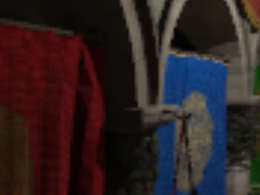
\includegraphics[width=.48\linewidth]{../../../output/rhi/sponza-detail-320.png}\hfill
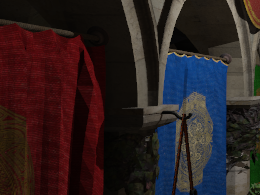
\includegraphics[width=.48\linewidth]{../../../output/rhi/sponza-detail-native.png}
\captionof*{figure}{同一旧版编辑器布局下的画质对照。左图用 320 像素宽的光照图放大，右图按面板原始分辨率绘制。两次面板均为 $948\times613$ 像素。左图源为 $320\times207$，右图源为 $948\times613$，裁切位置完全相同。}
\end{center}

默认设置下，转动或缩放相机时，场景继续显示选定的光照。若在组合光照 Lit 中开启「移动时仅算直接光」，移动期间会保留点光源的直接照明，停手后恢复所选效果。单独查看 DDGI 或 GTAO 时，移动镜头仍显示该项结果。镜头停下后，TAA 会继续合并几帧的颜色，让边缘更平滑。实时 DDGI 也会继续计算墙面收到的光。这些效果最多再画 32 帧，之后面板显示最后一张图。重新移动物体、修改灯光或调参数会恢复计算。

\clearpage
\section{移动相机与停手后的帧耗时}
这组历史测试记录了快速导航曾经省下多少时间。旧实现一移动就改画材质底色，停手后恢复光照。测试在 Sponza 中庭沿走廊缩放镜头，两轮使用三盏点光源、每方向两条射线的 DDGI、GTAO 与权重为 0.85 的 TAA。窗口客户区为 $1698\times984$，场景面板为 $948\times613$。运行环境为 Windows、Debug x64 和 GeForce RTX 5070 Ti Laptop GPU。

测试脚本向窗口送入 50 次滚轮输入，每次间隔 150 毫秒，每五步反向。第一轮关闭快速导航，第二轮打开。两轮都先让相机停在原处，等面板画完 32 帧，再滚动鼠标。表中第一行是关闭快速导航时测的，后三行是开启时测的。两轮都把计算光照所需的图像和表面数据放在显存里。

\begin{center}
\begin{tabularx}{\linewidth}{@{}Yrrr@{}}
\toprule
场景面板的工作 & 帧数 & 中位数 & 第 95 百分位\\\midrule
移动中持续计算完整光照 & 50 & 15.66 & 20.74\\
移动时只画材质底色 & 1819 & 4.15 & 5.78\\
停下后按面板大小重算光照 & 31 & 15.89 & 18.75\\
画完后继续显示同一张图 & 341 & 4.08 & 6.00\\
\bottomrule
\end{tabularx}
\captionof*{table}{一帧编辑器主循环的用时，单位为毫秒，含 CPU 工作、显卡同步与窗口呈现。「第 95 百分位」表示约 95\% 的帧在该时间内完成。原始时间线与可执行文件的 SHA-256 见 \path{output/profiling/compute-memory/final-navigation.json}。}
\end{center}

早期实现把计算所用的资源放在 CPU 可直接写入的内存里。同尺寸、同组光照选项下，移动时全光照一帧的中位数曾是 155.02 毫秒，输入多次合并，实际只记到 25 次镜头变化。这个历史数同时跨过了后来的编辑器改动。单独改变内存位置的对照见 \path{output/profiling/compute-memory/README.md}。

两种分辨率各测了一次。让镜头保持不动，等面板画完 32 帧，再间隔半秒截两张图。逐像素比较，两张图的颜色完全相同。要检查这 32 帧里墙面有没有闪烁，或转动镜头时物体边缘有没有拖影，还需要把正在绘制的帧分别截下来。

重新调整主窗口大小时，中间的视口会跟着变。一次实测把场景面板从 $948\times613$ 缩为 $775\times536$；预览的采样图按同一宽高比重建，模型、贴图和三角形的空间索引继续沿用。相机姿态和三盏灯都来自打开的场景。两次质量截图保存在 \path{output/rhi/}，相机、计时条件和两次截图的 SHA-256 见 \path{output/rhi/editor-quality.json}。

\clearpage
\section{中庭光照的一帧}
\begin{center}
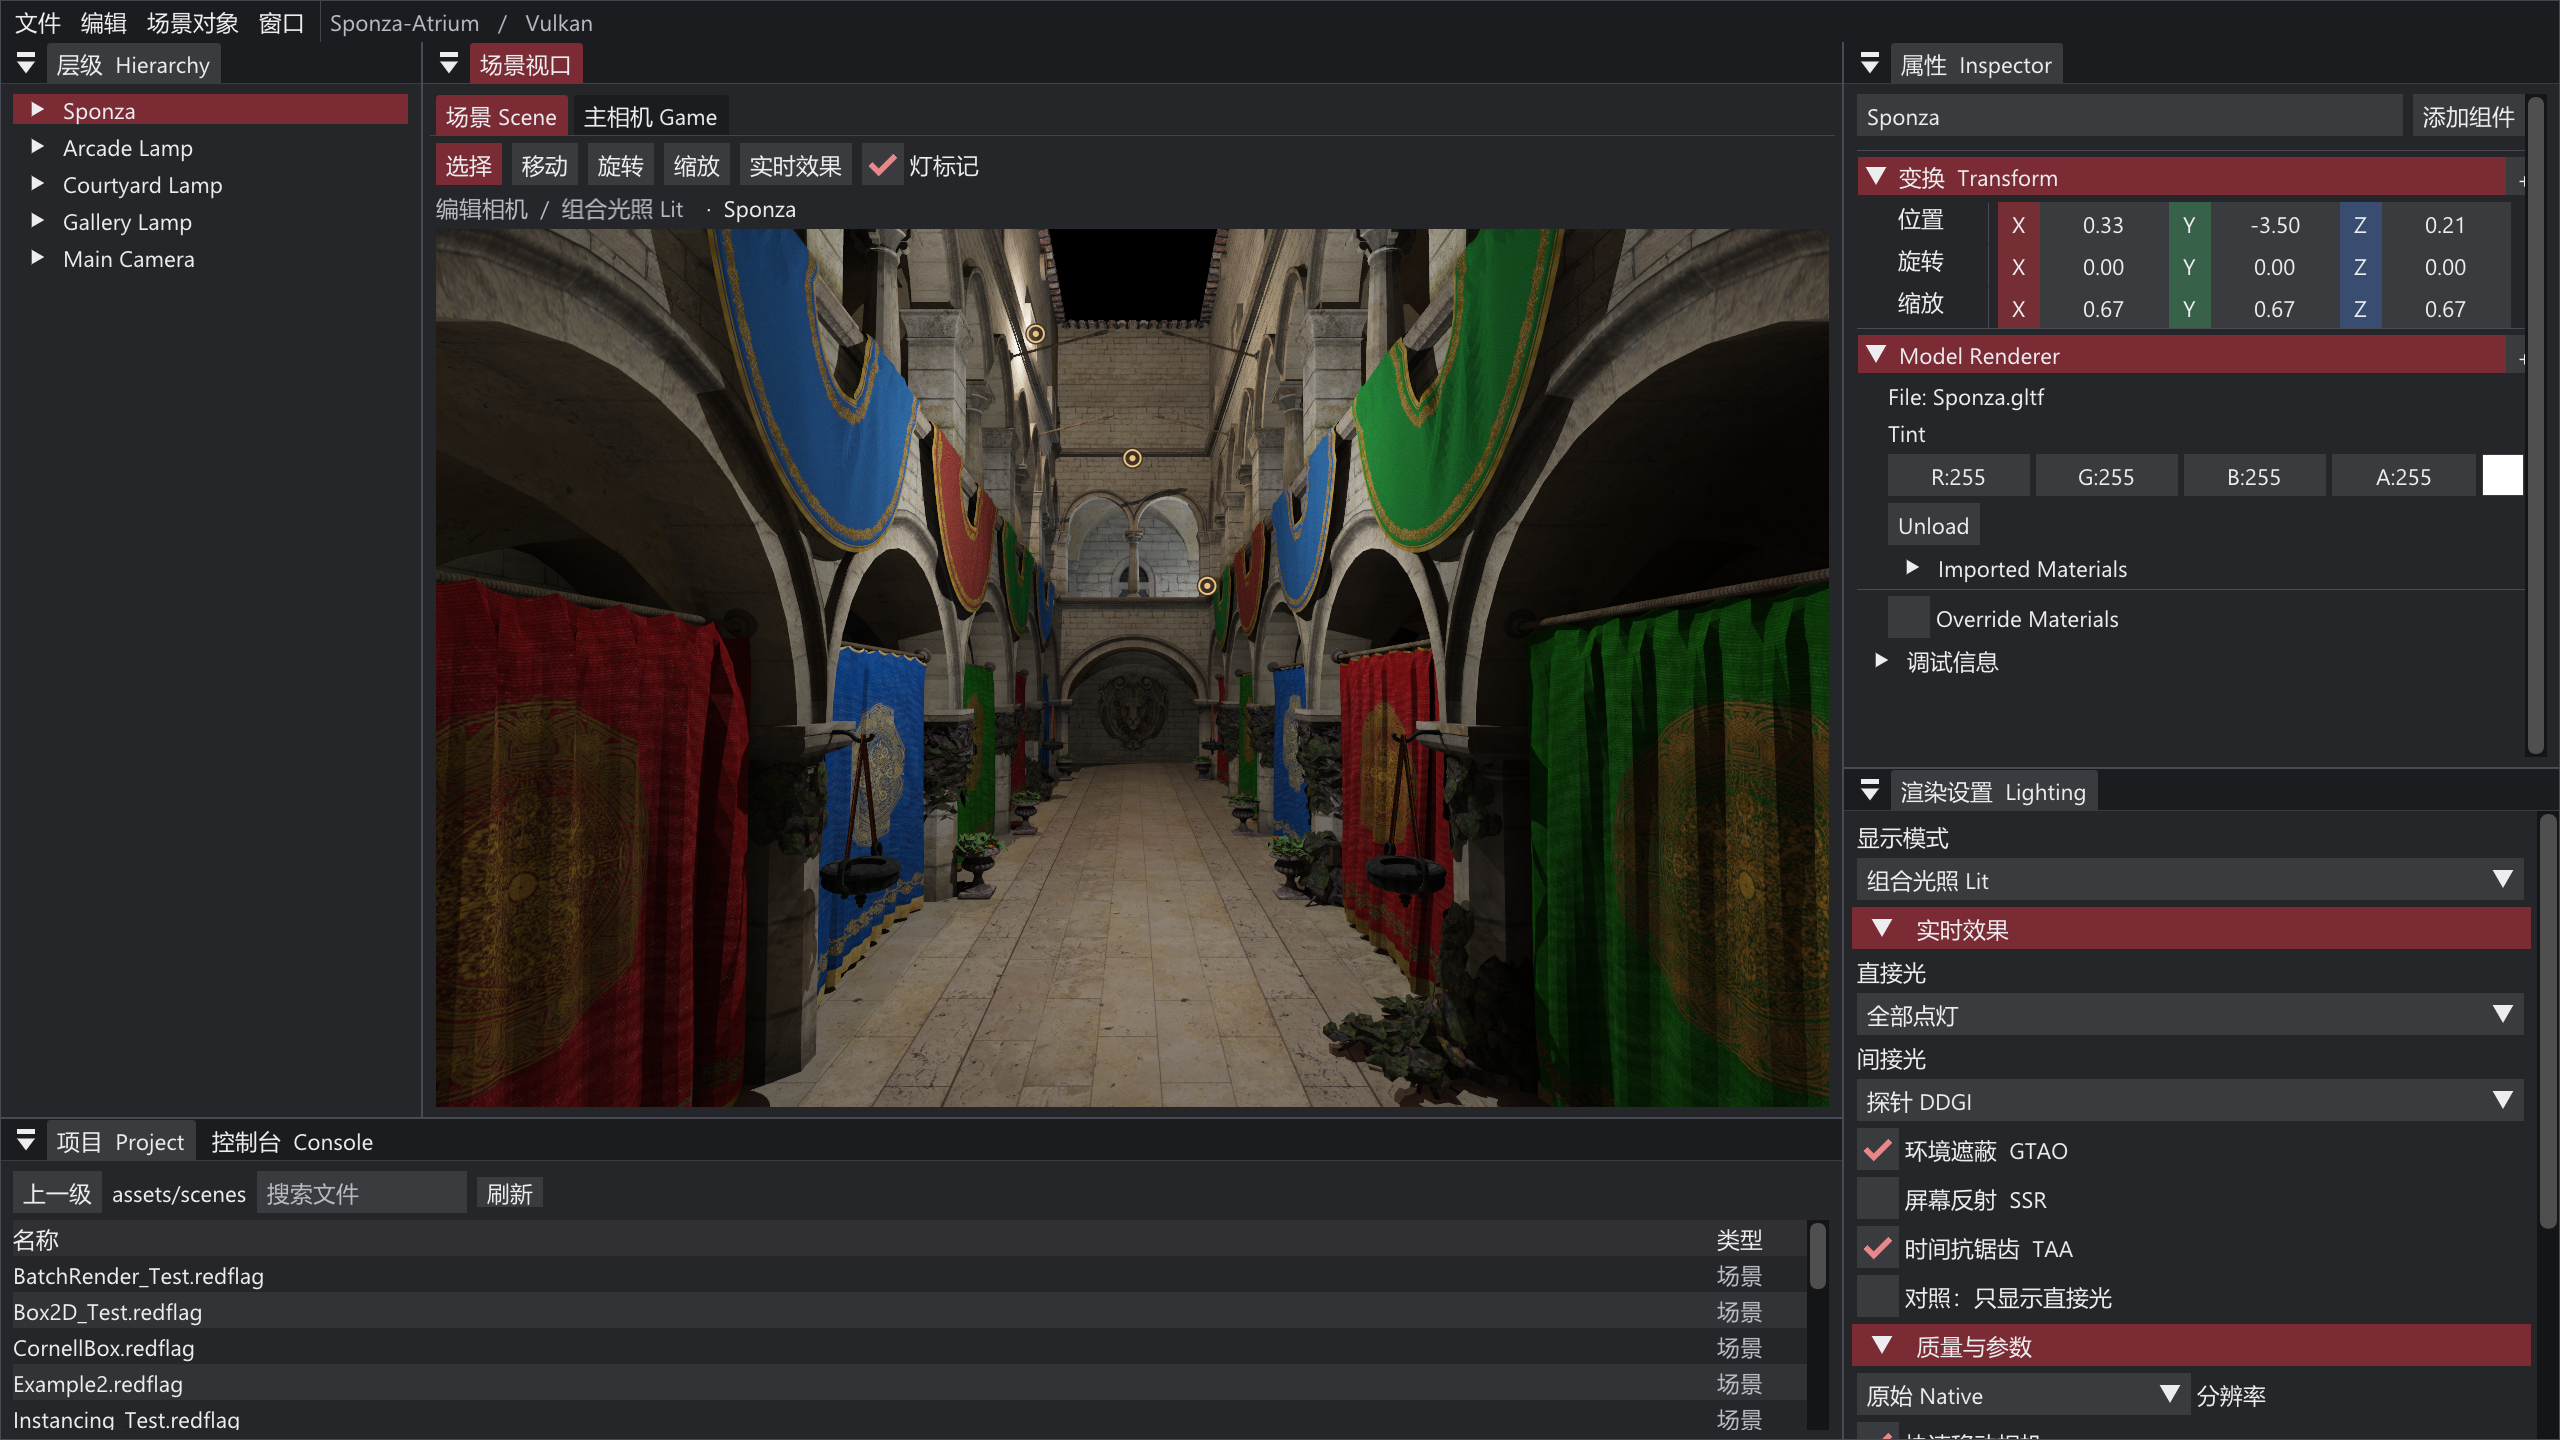
\includegraphics[width=.96\linewidth]{../../../output/rhi/editor-sponza-rdc.png}
\captionof*{figure}{RenderDoc 1.47 回放第 10 帧。窗口为 $2560\times1440$ 像素，中庭用三个点光源、DDGI、GTAO 和 TAA 绘制，视口为 $1393\times878$。截图保留捕获时的布局和标签。}
\end{center}

在事件列表中从上往下看，事件 11 至 108 有九次计算。前五次处理场景表面与光照，后四次分别计算 GTAO、合并直接光与间接光、累积 TAA 和生成供界面显示的图。双击事件 108 时，场景颜色已经算好，此时尚未把面板画到窗口。

接下来，事件 120 开始的光栅绘制将中庭的 103 个网格绘制请求写入底色图和实体编号图。查看事件 128 的颜色输出能看到两张同样大小的图，第二张的格式为 \code{R32\_SINT}，保存鼠标能选中的实体编号。事件 640 开始绘制界面，最后一次绘制在事件 712 结束。ImGui 用了 22 次绘制，将光照图与层级、属性等控件排进同一张窗口图。

本地帧文件为 \path{output/captures/local/Forge-Sponza-Lit-10.rdc}，约 700 MB，不随 Git 分发。仓库中的 \path{output/rhi/editor-sponza-events.json} 记录了原件校验值、事件编号、截图和复现步骤。要看显卡怎样算光照，请在前 32 帧内截帧。镜头停着且这 32 帧已经画完时，面板只显示最后一张图。回放和导出的截图用于核对执行顺序，时间仍以上一页的编辑器主循环实测为准。

\clearpage
\section{挂毯的颜色、深度和实体编号}
场景面板里的红挂毯有金色花纹。图中 A 在花纹附近，B 在拱顶露出的背景上。四张图取自上一页的同一帧，同一个字母始终指向同一个像素。先看上排，底色图留下了金色花纹，光照图又让走廊深处暗了下来。编辑器显示 Lit 时用右上图，切换材质底色时用左上图。

\begingroup
\newcommand{\attachment}[2]{%
  \begin{minipage}{.484\linewidth}
  {\noindent\sffamily\bfseries\small\color{Teal}#2\par}
  \noindent\begin{tikzpicture}
    \node[inner sep=0] (im) {\includegraphics[width=\linewidth]{figures/sponza-attachments/#1.png}};
    \foreach \x/\y/\letter in {.0575/.316/A,.4986/.9675/B}{
      \coordinate (point) at ($(im.south west)!\x!(im.south east)$);
      \coordinate (high) at ($(im.south west)!\y!(im.north west)$);
      \node[circle,inner sep=0pt,minimum size=3.4mm,font=\sffamily\bfseries\tiny,
        draw=white,fill=Ink,text=white,line width=.45pt] at (point |- high) {\letter};
    }
  \end{tikzpicture}
  \end{minipage}}
\noindent\attachment{color}{材质底色}\hfill\attachment{lit}{编辑器显示的光照}
\par\smallskip
\noindent\attachment{depth}{深度　近处亮，远处暗}\hfill\attachment{entity}{实体编号　青色为中庭，米色为背景}
\par
\endgroup


遮挡和拾取各要回答另一个问题。显卡画到 A 时，用深度判断挂毯和它后面的墙哪一面更靠前。为了能在纸上看清远近，左下将深度 $0.955$ 到 $1$ 之间的数值展开成从白到黑。A 的深度约为 $0.965$，B 保留背景值 $1$。这些数值来自投影后的深度图，和相机距离的米数不同。

右下只给两种编号上色。挂毯、石柱和地砖随中庭模型一起导入，尽管外观不同，点击它们都选中编号 4。顶部的背景仍是 $-1$，那里没有可选中的模型。调整灯光时，右上图的颜色可以改变，点击 A 仍会选中中庭。

\readings{RedflagForge，Sponza 中庭，RenderDoc 1.47，第 10 帧。光照输出由事件 108 写入，四张图均在最后一次场景绘制（事件 638）之后读取，原始尺寸 $1393\times878$。}


\clearpage
\section{颜色图怎样出现在场景面板里}
下面是打开项目自带 \path{assets/scenes/CornellBox.redflag} 后的实际编辑器画面。层级面板里，红墙是 \code{LeftWall\_Red}，绿墙是另一个实体。这张截图来自最初接入 Vulkan 的版本，当时只显示材质颜色，因此房间内部的两只浅色箱子与地面的明暗很接近。

\begin{center}
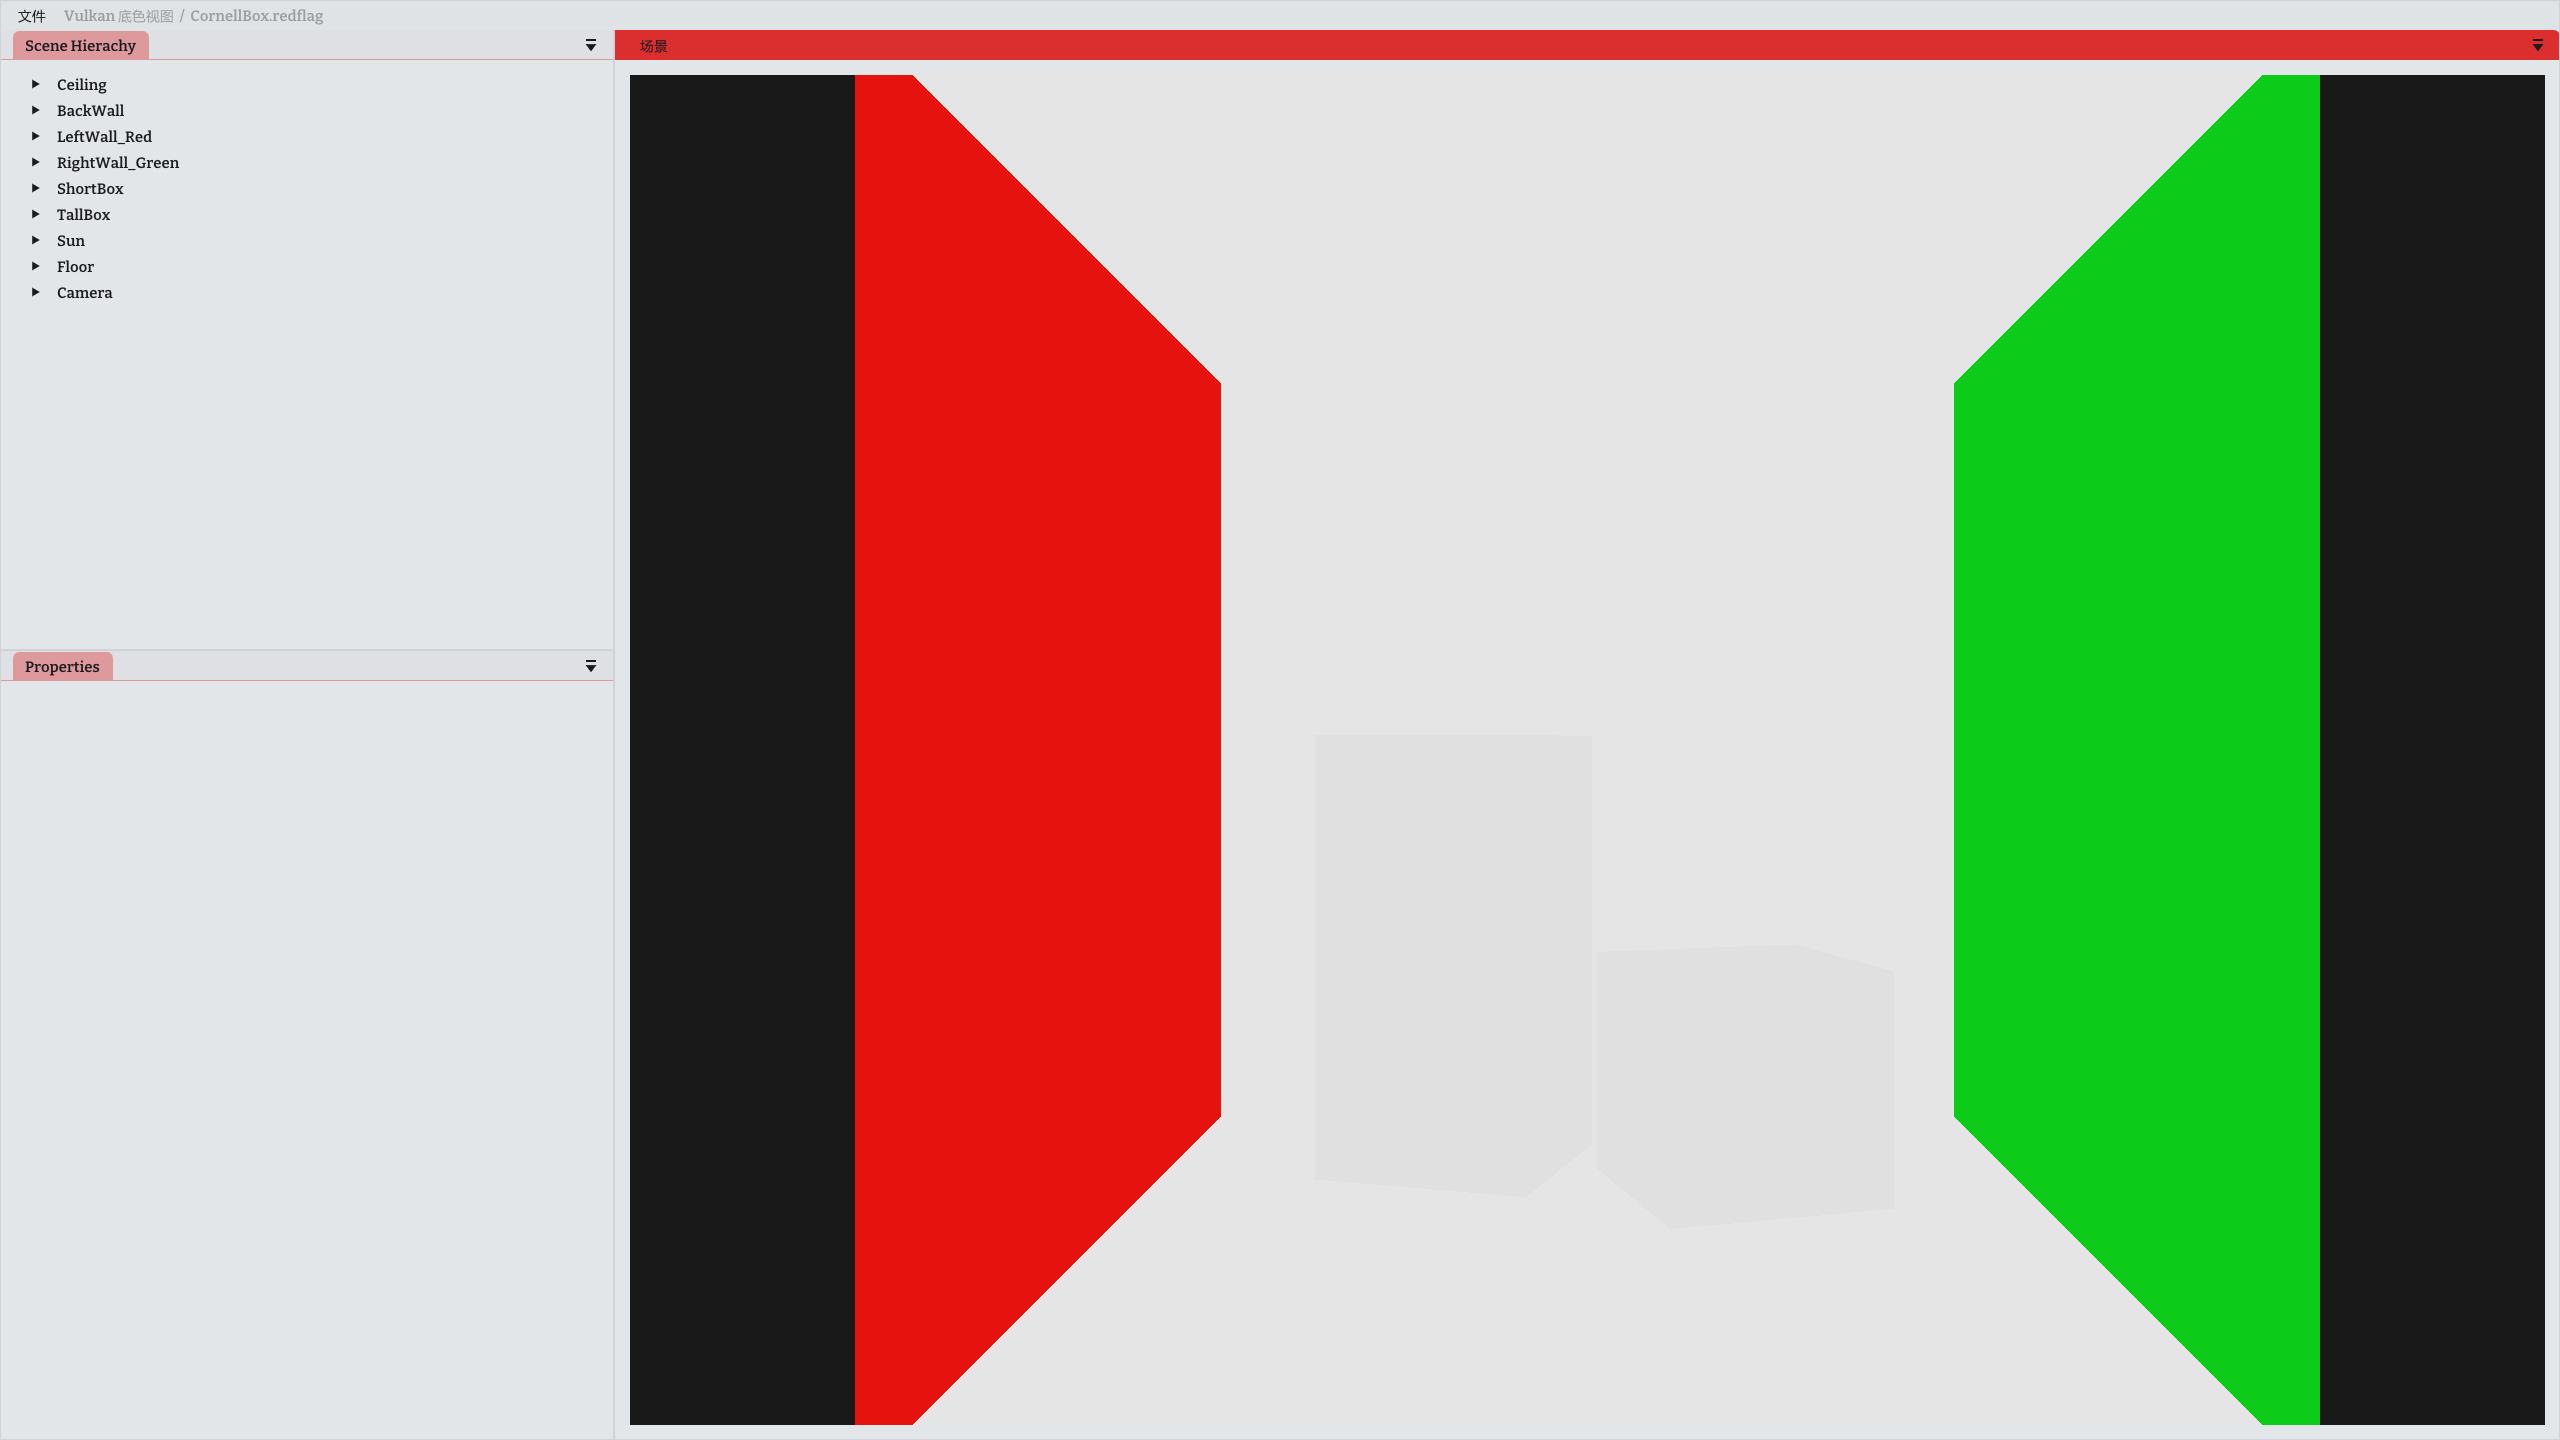
\includegraphics[width=.97\linewidth]{../../../output/rhi/forge-cornell-window.png}
\captionof*{figure}{RenderDoc 回放正式编辑器第 66 帧，窗口为 $2560\times1440$ 像素。七次网格绘制在事件 49 结束，随后五次 ImGui 绘制把右侧场景和左侧工具面板合到窗口图上，最后一次为事件 72。}
\end{center}

每帧，编辑器先根据右侧面板的实际像素尺寸选好绘制目标。\code{BeginScene} 清除上次留下的颜色、实体编号和深度。\code{SceneRenderer::DrawGeometry} 将模型画进这些图，\code{EndScene} 结束这次场景绘制。随后 ImGui 从颜色图读取像素，把它和左边的实体列表一起画进窗口图像，最后才轮到窗口呈现。面板只占窗口的一部分，这正是要保留两张不同颜色图的原因。

点选时读另一项结果。编辑器将鼠标位置减去场景图的左上角，再按实际像素尺寸换算。在 Vulkan 路径里，图的左上角就是像素 $(0,0)$。\code{ReadPixel} 返回该位置上一次已提交的实体编号；层级面板拿这个编号去当前场景中找实体。背景保留清除时写入的 $-1$，点击空处会清掉选中状态。

\clearpage
\section{资源创建与场景绘制}\label{impl:objects}
导入一扇带木纹的门时，模型加载器已经读出两组数组：顶点写明门板各个角的位置和贴图坐标，索引写明哪些角连成三角形。它仍然调用项目原有的 \code{Mesh::Create}。\code{Mesh} 从顶点算出自己的包围盒，再通过当前 \code{RenderDevice} 创建显卡上的几何。模型保存返回的对象，下一帧即使相机换了位置，这些顶点和索引仍可使用。

\codewhere{源码}{Redflag/src/Redflag/Renderer/Mesh.cpp}{Mesh::Mesh}
\begin{lstlisting}
(*@\rhicomment{// 几何随网格保存，移动相机时继续用这一份。}@*)
m_Geometry = RenderDevice::Get().CreateMesh(vertices, indices);
\end{lstlisting}

对 OpenGL，设备把顶点布局、顶点缓冲和索引缓冲关联到一个顶点数组对象。对 Vulkan，后端先把原始数值写入 CPU 能访问的暂存缓冲区，录下复制命令，把同样的数值写到绘制使用的缓冲区。加载器拿到创建结果以后可以释放原数组。底色图也遵循这项约定，因此 \code{CreateTexture} 的接口注释说明了像素的顺序，以及调用者可以在什么时候释放它们。

\subsection{材质由场景选，后端接收这次绘制}
如果只给一扇门换颜色，编辑器会在这个实体上保存覆盖材质。\code{SceneRenderer} 遍历场景时优先选它；没有覆盖时沿用模型部件自带的材质。部件的顶点先放进模型，再随整扇门进到世界中。代码把实体矩阵乘在部件矩阵左边。现有 OpenGL 完整渲染和 Vulkan 底色视图共用这段收集逻辑。前者把网格交给 \code{Renderer3D} 继续做可见性判断和合批，后者调用下面的接口。

\codewhere{源码}{Redflag/src/Redflag/Renderer/SceneRenderer.cpp}{SceneRenderer::DrawGeometry}
\begin{lstlisting}
(*@\rhicomment{// world 定位这个部件，id 让编辑器能找回实体。}@*)
commands.DrawIndexed(mesh->GetGeometry(), texture, viewProjection,
                     world, material->BaseColor, id, surface);
\end{lstlisting}

设备接口在 \path{Renderer/RHI/RenderDevice.h}，绘制接口在同目录的 \path{CommandList.h}。前者接收顶点或像素，返回可以保留的资源；后者接收本次使用的资源和数值。网格、贴图、材质仍各自在原有资源头文件里。要改材质选择，可以从 \code{SceneRenderer} 找；要查 GPU 最终收到的指令，则看 \code{VulkanDraw::DrawIndexed}。

\clearpage
\section{用一个像素检查绘制}\label{impl:pixels}
一块蓝色方形放在绿色方形的前面。测试故意先画近处的蓝色，再画远处的绿色。如果只看最后一次绘制，重叠处应当变绿。打开深度测试后，远处片元未能通过测试，这里的颜色和拾取编号都会保留近处方形的值。下面是从本项目的 Vulkan 帧直接导出的颜色图。

\begin{center}

\includegraphics[width=.40\linewidth]{../../../output/rhi/mesh-depth-color.png}
\captionof*{figure}{RenderDoc 1.47 回放，原图 $32\times16$ 像素。蓝面为实体 17，绿面为实体 42。两次索引绘制分别是事件 13 和 18，每次读六个索引。}
\end{center}

\noindent\begin{tabularx}{\linewidth}{@{}L{33mm}L{28mm}L{45mm}Y@{}}
\toprule
从左上角量起 & 采样位置 & 读回的 RGB & 实体编号\\\midrule
$(8,4)$ & 只有近面 & $(43,82,231)$ & 17\\
$(24,4)$ & 只有远面 & $(31,208,67)$ & 42\\
$(16,4)$ & 两面重叠 & $(43,82,231)$ & 17\\
$(16,12)$ & 背景 & 清除时的颜色 & $-1$\\
\bottomrule
\end{tabularx}

两个后端的命令列表读取同一份测试输入。四种颜色来自一张 $2\times2$ 的真实贴图，两个网格的贴图坐标分别指向蓝色和绿色。程序先在 $32\times16$ 的目标上连续画三帧，再换成 $64\times32$ 画三帧，分别读取对应位置。两种尺寸的 OpenGL 和 Vulkan 结果都通过了检查。复现入口是仓库根目录的 \path{tests/run_rhi_tests.cmd}。

\subsection{怎样解释这次截帧}
本机 RTX 5070 Ti Laptop GPU 运行原生 Vulkan 测试时，Khronos 验证层未报告错误。对同一份捕获额外开启 RenderDoc 的回放校验，打开帧时事件 4 出现四条图像布局消息；再定位两个绘制事件没有新增消息。这一差异尚待定位。两份原始捕获保存在仓库的 \path{output/captures} 中，可用 RenderDoc 1.47 回放。表中的实测值可以用来回归颜色、遮挡和点选，不能据此推算 GPU 用时。

\clearpage
\section{视口尺寸与图像寿命}\label{impl:fix}
最初接入时，离屏测试已经能画对两个方形，正式编辑器却在打开 Cornell Box 时触发了相机投影断言。测试自己指定投影矩阵，编辑器从场景文件恢复相机。反序列化刚添加相机组件，场景就会用当前宽高设置它的投影。此时若宽和高还都是零，宽高比就算不出来。

\codewhere{旧调用顺序 · 伪代码}{RedflagForge/src/VulkanForgeLayer.cpp}{VulkanForgeLayer::OpenScene}
\begin{lstlisting}
(*@\rhicomment{// 旧版本在面板宽高仍为零时读入了场景相机。}@*)
SceneSerializer(scene).Deserialize(path);
\end{lstlisting}

\codewhere{源码}{RedflagForge/src/VulkanForgeLayer.cpp}{VulkanForgeLayer::OpenScene}
\begin{lstlisting}
(*@\rhicomment{// 新视口还没有尺寸时，先借用窗口宽高计算投影。}@*)
auto extent = m_Draw->GetExtent();
if (extent.width == 0)
    extent = GetWindowContext().GetExtent();
scene->OnViewportResize(extent.width, extent.height);

if (!SceneSerializer(scene).Deserialize(path.string()))
{
    Report("Could not open scene: " + path.u8string());
    return;
}
\end{lstlisting}

首次开场景时，ImGui 还没有排出场景面板，但窗口已经有可用的像素尺寸。先把它交给场景，相机组件就能正常创建。面板完成布局后，再用面板的实际尺寸更新场景。这处修改放在打开场景的入口，相机仍按原来的规则计算投影。

\subsection{当前实现怎样保留已经提交的数据}
移动一个物体后，Vulkan 将新的矩阵、底色和实体编号随这条绘制命令写入少量常量\termenglish{push constants}。网格与贴图继续共用。后端轮流使用两份工作帧，各自保留该帧用到的网格与贴图引用。等对应的围栏通知 CPU 绘制完成，这一份才可重新录制。

拖大面板时，当前实现先建立新图，再等显卡用完旧图才更换。鼠标点选也采用同步读回，只在点击时等一个像素的结果。这样第一次接入时容易检查图像究竟来自哪帧，代价是这些操作可能使 CPU 等待。后文关于延后回收与异步拾取的设计，可以在保留本次像素测试的基础上继续实现和计时。

\readings{\path{RedflagForge/src/VulkanForgeLayer.cpp}\quad
\path{Redflag/src/Redflag/Scene/Scene.cpp}\quad
\refitem{https://docs.vulkan.org/guide/latest/push_constants.html}{Khronos · 随命令记录常量}}
